%\documentstyle[epsf,twocolumn]{jarticle}       %LaTeX2.09仕様
\documentclass[twocolumn]{jarticle}     %pLaTeX2e仕様

%\usepackage[backend=bibtex, style=numeric]{biblatex}
%\addbibresource{sankou.bib}
%%%%%%%%%%%%%%%%%%%%%%%%%%%%%%%%%%%%%%%%%%%%%%%%%%%%%%%%%%%%%%
%%
%%  基本 バージョン
%%
%%%%%%%%%%%%%%%%%%%%%%%%%%%%%%%%%%%%%%%%%%%%%%%%%%%%%%%%%%%%%%%%
\setlength{\topmargin}{-45pt}
%\setlength{\oddsidemargin}{0cm}
\setlength{\oddsidemargin}{-7.5mm}
%\setlength{\evensidemargin}{0cm}
\setlength{\textheight}{24.1cm}
%setlength{\textheight}{25cm}
\setlength{\textwidth}{17.4cm}
%\setlength{\textwidth}{172mm}
\setlength{\columnsep}{11mm}

\setlength{\intextsep}{8pt}
\setlength{\textfloatsep}{8pt}
\setlength{\floatsep}{1pt}

\kanjiskip=.07zw plus.5pt minus.5pt



%【節がかわるごとに(1.1)(1.2) …(2.1)(2.2)と数式番号をつけるとき】
%\makeatletter
%\renewcommand{\theequation}{%
%\thesection.\arabic{equation}} %\@addtoreset{equation}{section}
%\makeatother

%\renewcommand{\arraystretch}{0.95} 行間の設定

\usepackage[dvipdfmx]{graphicx}   %pLaTeX2e仕様(\documentstyle ->\documentclass)
\usepackage{scalefnt}
\usepackage{bm}
\usepackage{here}
\usepackage{url}
\usepackage{amsmath}
\usepackage{amsfonts}
\usepackage[subrefformat=parens]{subcaption}
\captionsetup{compatibility=false}
%%%%%%%%%%%%%%%%%%%%%%%%%%%%%%%%%%%%%%%%%%%%%%%%%%%%%%%%
\usepackage{comment}
\usepackage{subcaption}
\usepackage{multirow}
\usepackage{nidanfloat}
\usepackage[dvipdfmx]{hyperref}

\usepackage[normalem]{ulem}
\useunder{\uline}{\ul}{}

\begin{document}

\twocolumn[
\noindent
\hspace{1em}

令和2年5月13日(水) ゼミ資料
\hfill
\ \ B4 高山 裕成

\vspace{2mm}
\hrule
\begin{center}
{\Large  進捗報告}
\end{center}
\hrule
\vspace{3mm}
]

\section{あらすじ}
BERT\cite{BERT} を全層 fine-tuning したらダメだった.

% \footnotesize
\section{進捗}

\begin{itemize}
  \item BERT の fine-tuning やり直し (固定, 最後のレイヤーのみ)
  \item 岡田先生の課題
\end{itemize}

\section{BERT fine-tuning やり直し}

先週行った実験について, 最終レイヤーのみのチューニング (BERT last layer), またはすべてのパラメータを固定させる (BERT fixed) 条件で BERT fine-tuning を追加で行った.
識別器としては 3 層 MLP を用いた.

\subsection{結果}
実験の結果を表\ref{tab:result} に示す.
表より, BERT の 最後のレイヤーのみをチューニングすることでより汎化性能が高まることが分かった. 学習曲線は資料の終わりに添付してある.

\begin{table*}[!b]
\begin{center}
\caption{result}
\scalebox{0.65}{
\begin{tabular}{lccccccccccccccc|ccc}
  \hline
  \multicolumn{1}{c}{\multirow{2}{*}{model}} & \multicolumn{3}{c}{ギャグ} & \multicolumn{3}{c}{少女漫画} & \multicolumn{3}{c}{少年漫画} & \multicolumn{3}{c}{青年漫画} & \multicolumn{3}{c|}{萌え系} & \multicolumn{3}{c}{5タッチ平均} \\
  \multicolumn{1}{c}{} & \multicolumn{1}{c}{Acc} & \multicolumn{1}{c}{Recall} & \multicolumn{1}{c}{F1} & \multicolumn{1}{c}{Acc} & \multicolumn{1}{c}{Recall} & \multicolumn{1}{c}{F1} & \multicolumn{1}{c}{Acc} & \multicolumn{1}{c}{Recall} & \multicolumn{1}{c}{F1} & \multicolumn{1}{c}{Acc} & \multicolumn{1}{c}{Recall} & \multicolumn{1}{c}{F1} & \multicolumn{1}{c}{Acc} & \multicolumn{1}{c}{Recall} & \multicolumn{1}{c|}{F1} & \multicolumn{1}{c}{Acc} & \multicolumn{1}{c}{Recall} & \multicolumn{1}{c}{F1} \\ \hline
  d2v (manga109) + 3MLP & 0.652 & 0.300 & 0.207 & 0.537 & 0.632 & 0.608 & 0.625 & 0.667 & 0.400 & 0.662 & 0.357 & 0.312 & 0.563 & 0.364 & 0.364 & 0.608 & 0.464 & 0.378 \\
  d2v (wiki) + 3MLP & 0.652 & 0.200 & 0.148 & 0.433 & 0.447 & 0.472 & 0.781 & 0.500 & {\ul 0.462} & {\ul 0.815} & 0.643 & {\ul 0.600} & 0.531 & 0.409 & 0.375 & 0.642 & 0.440 & 0.411 \\
  d2v (manga109 + wiki) + 3MLP & 0.621 & 0.200 & 0.138 & {\ul 0.612} & 0.579 & {\ul 0.629} & 0.750 & 0.250 & 0.273 & 0.708 & 0.429 & 0.387 & 0.531 & 0.455 & 0.400 & 0.644 & 0.382 & 0.365 \\
  BERT (All Layers) + Linear & 0.803 & 0.000 & 0.000 & 0.433 & 0.000 & 0.000 & 0.188 & 1.000 & 0.316 & 0.215 & 1.000 & 0.354 & 0.344 & 1.000 & {\ul 0.512} & 0.397 & 0.600 & 0.236 \\ \hline
  BERT (Last Layer) + 3MLP & {\ul 0.833} & 0.400 & 0.421 & 0.567 & 0.579 & 0.603 & {\ul 0.797} & 0.083 & 0.133 & 0.800 & 0.357 & 0.435 & {\ul 0.656} & 0.455 & 0.476 & {\ul 0.731} & 0.375 & {\ul 0.414} \\
  BERT (Fixed) + 3MLP & 0.818 & 0.500 & {\ul 0.455} & 0.463 & 0.421 & 0.471 & 0.766 & 0.000 & 0.000 & 0.769 & 0.429 & 0.444 & 0.625 & 0.409 & 0.429 & 0.688 & 0.352 & 0.360 \\ \hline
  ベースライン & \multicolumn{1}{c}{0.85} & \multicolumn{1}{c}{0} & \multicolumn{1}{c}{0} & \multicolumn{1}{c}{0.43} & \multicolumn{1}{c}{0} & \multicolumn{1}{c}{0} & \multicolumn{1}{c}{0.81} & \multicolumn{1}{c}{0} & \multicolumn{1}{c}{0} & \multicolumn{1}{c}{0.78} & \multicolumn{1}{c}{0} & \multicolumn{1}{c}{0} & \multicolumn{1}{c}{0.66} & \multicolumn{1}{c}{0} & \multicolumn{1}{c|}{0} & \multicolumn{1}{c}{0.71} & \multicolumn{1}{c}{0} & \multicolumn{1}{c}{0}
\end{tabular}
\label{tab:result}
}
\end{center}
\end{table*}

\section{岡田先生課題}
日本語カスタマーレビューデータセットのネガポジ分類 (0: 不評, 1: 好評) を行った. MeCab で分かち書きし, BERT への入力の都合上長すぎる文章は除いた. 訓練データセットのうち, 20\% を検証用データセットとし, 検証用データの accuracy が最大となるエポックでのモデルを採用し, テストデータセットによって評価した. 識別器としては 3 層 MLP を用いて, 同様に BERT の最終レイヤーのみのチューニング (BERT last layer), またはすべてのパラメータを固定させる (BERT fixed) 条件で実験を行った. データ数は表\ref{table:data} , 学習パラメータは図\ref{table:ex_para} に示す.

\begin{table}
\caption{data}
\label{table:data}
\centering
\begin{tabular}{lccl}
\hline
 & label 0 & label 1 & 合計 \\ \hline
train $+$ valid & 1970 & 1998 & 3968 \\
test & 973 & 995 & 1968 \\ \hline
合計 & 2943 & 2993 & 5936 \\ \hline
\end{tabular}
\end{table}


\begin{table}
\caption{学習パラメータ}
\label{table:ex_para}
\centering
\begin{tabular}{|c||c|c|}
\hline
& \multicolumn{2}{|c|}{実験} \\ \hline
epoch & \multicolumn{2}{|c|}{100}  \\ \hline
batch size & \multicolumn{2}{|c|}{16} \\ \hline
loss function & \multicolumn{2}{|c|}{Cross Entropy Loss} \\ \hline
optimizer & \multicolumn{2}{|c|}{Adam} \\ \hline
\end{tabular}
\end{table}

\subsection{結果}
結果を表\ref{table:result_negaposi} に示す. 学習曲線は資料の終わりに添付してある.

\begin{table}[]
\caption{ネガポジ実験結果}
\label{table:result_negaposi}
\centering
\begin{tabular}{l|cc}
\hline
 & Acc & F1 macro \\ \hline
BERT fixed & 0.728 & 0.722 \\
BERT last layer & 0.793 & 0.793 \\ \hline
ベースライン & 0.5 & 0.5\\ \hline
\end{tabular}
\end{table}

\section{今後の実験予定}
\begin{itemize}
  \item 正例に指定する感情ラベルを変えて実験. (ニュートラル, 驚愕, 喜楽)
  \item 直前 n - 1 文 を考慮した n 文を入力して末尾入力の感情推定をする.
  \item 森先生と大工大の上野先生に 30 話まであるらしい追加データをお願いする.
  \item Data Augmentation の手法の改善案.
\end{itemize}

\section{usagi server の不具合?}
\begin{verbatim}
  2020-05-20 00:56:45.899608: W tensorflow/stream_executor/platform/default/dso_loader.cc:55]
  Could not load dynamic library 'libnvinfer.so.6';
  dlerror: libnvinfer.so.6: cannot open shared object file:
  No such file or directory

  2020-05-20 00:56:45.899732: W tensorflow/stream_executor/platform/default/dso_loader.cc:55]
  Could not load dynamic library 'libnvinfer_plugin.so.6';
  dlerror: libnvinfer_plugin.so.6: cannot open shared object file:
  No such file or directory

  2020-05-20 00:56:45.899740: W tensorflow/compiler/tf2tensorrt/utils/py_utils.cc:30]
  Cannot dlopen some TensorRT libraries.
  If you would like to use Nvidia GPU with TensorRT,
  please make sure the missing libraries mentioned above are installed properly.

\end{verbatim}

TensorRT のライブラリが消えたのが原因?

よく分かりません.

\bibliographystyle{unsrt}
\bibliography{sankou}

\clearpage
\begin{figure*}[h]
  \begin{center} %センタリングする
    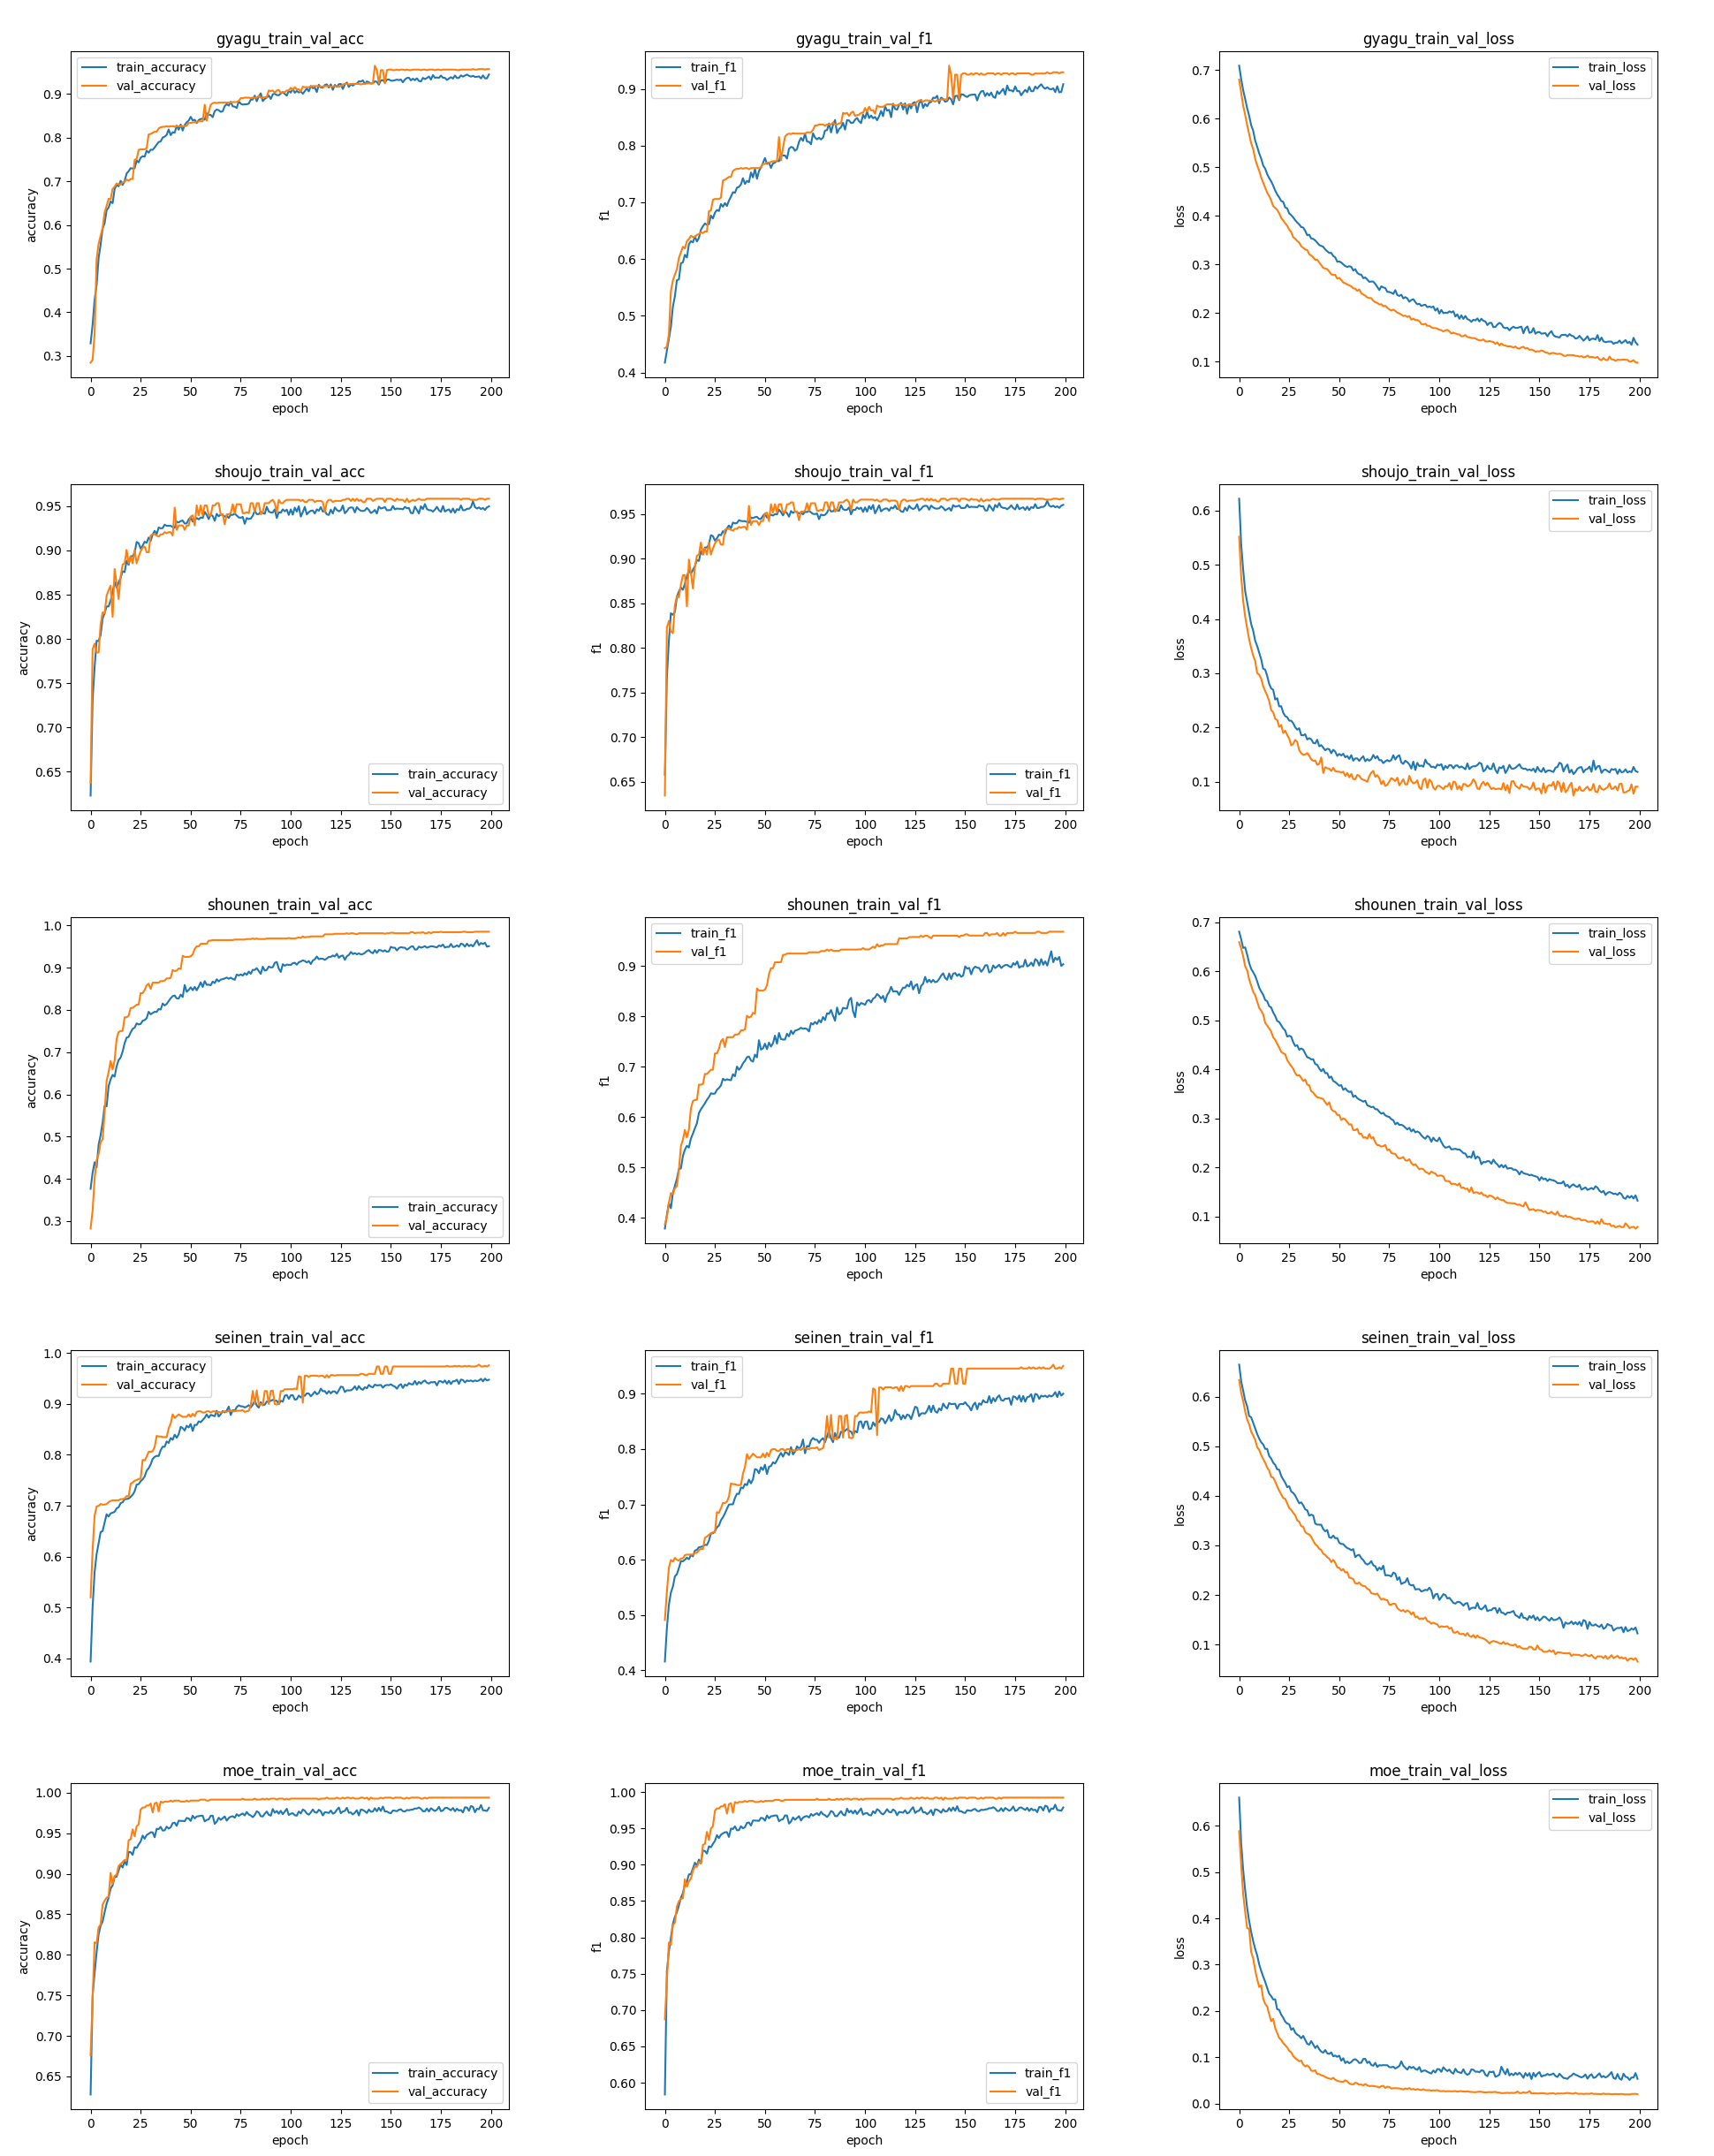
\includegraphics[width=14.0cm]{bert_fixed.png}
    \caption{manga bert fixed} %タイトルをつける
    \label{fig:manga_bert_fixed} %ラベルをつけ図の参照を可能にする
  \end{center}
\end{figure*}

\clearpage
\begin{figure*}[h]
  \begin{center} %センタリングする
    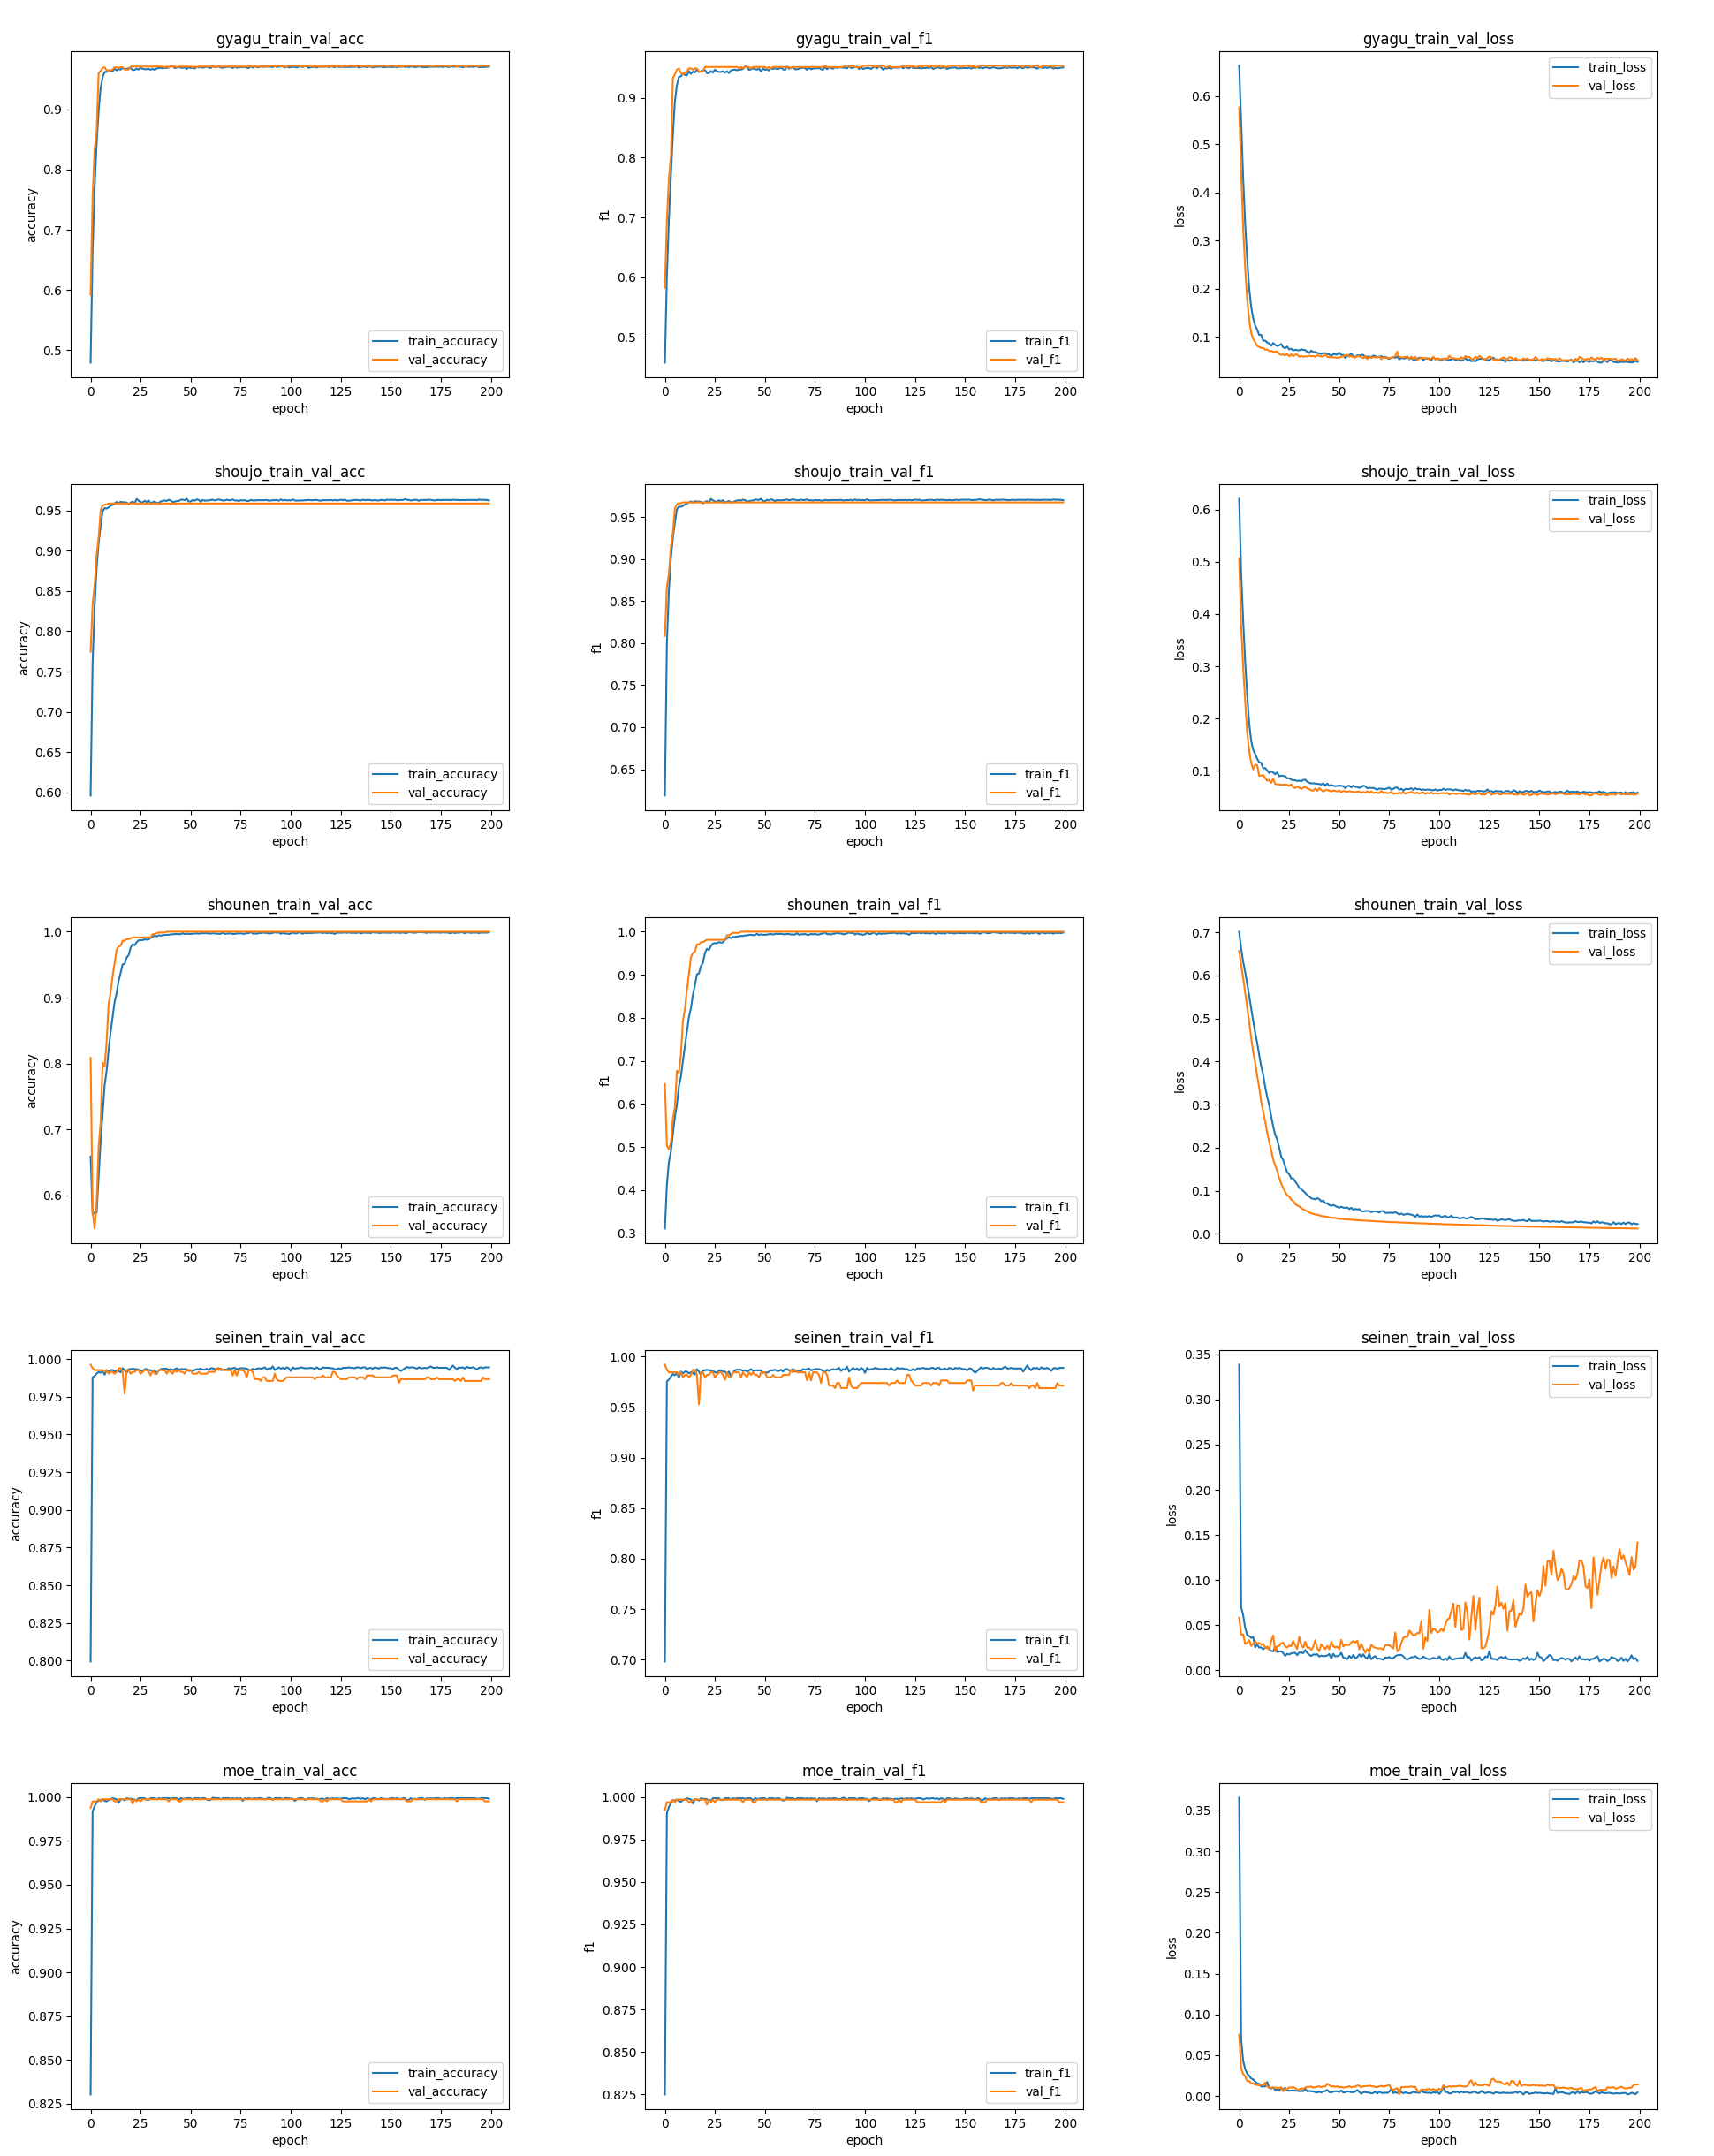
\includegraphics[width=14.0cm]{bert_last_layer.png}
    \caption{manga last layer} %タイトルをつける
    \label{fig:manga_last_layer} %ラベルをつけ図の参照を可能にする
  \end{center}
\end{figure*}

\clearpage
\begin{figure*}[h]
  \begin{center} %センタリングする
    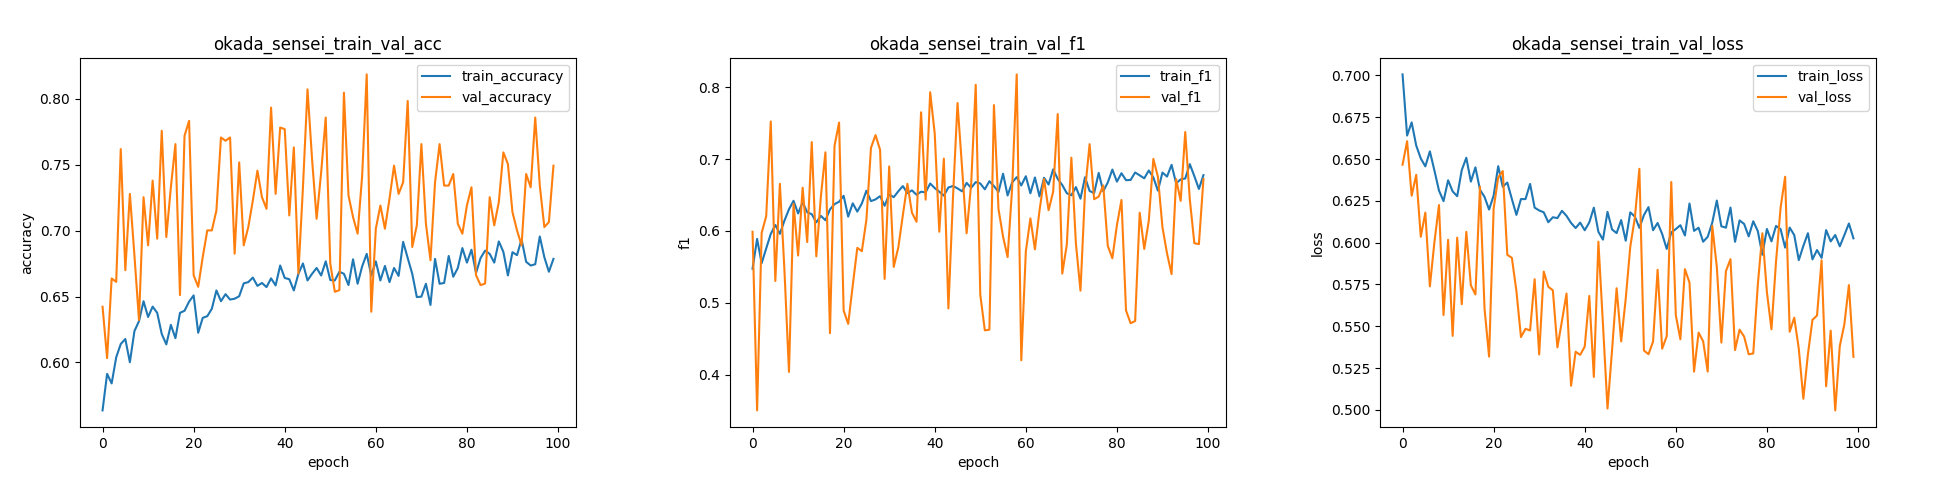
\includegraphics[width=14.0cm]{oakada_sensei_fixed.png}
    \caption{okadasensei bert fixed} %タイトルをつける
    \label{okadasensei_bert_fixed} %ラベルをつけ図の参照を可能にする
  \end{center}
\end{figure*}

\begin{figure*}[h]
  \begin{center} %センタリングする
    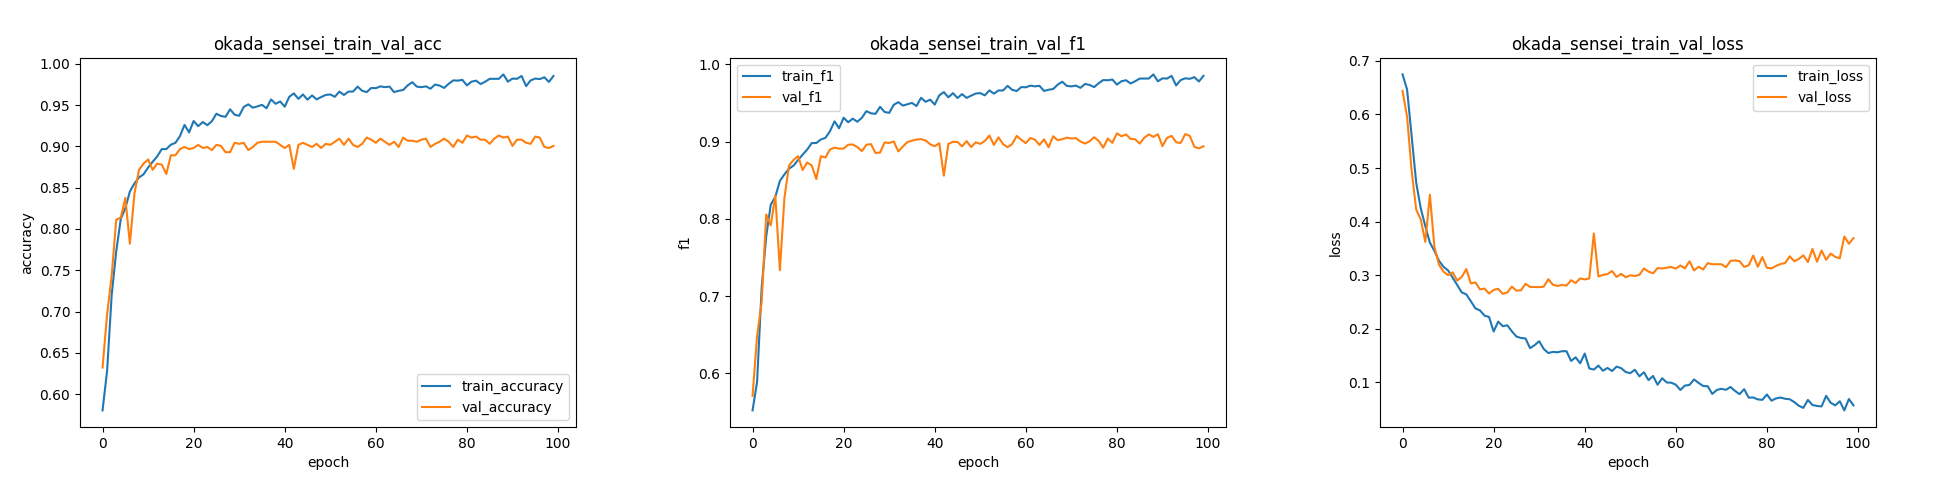
\includegraphics[width=14.0cm]{okada_sensei_last_layer.png}
    \caption{okadasensei bert last layer} %タイトルをつける
    \label{okadasensei_bert_last_layer} %ラベルをつけ図の参照を可能にする
  \end{center}
\end{figure*}

\end{document}
